% ---------------------------------------------------------------------------------------------
%  An AI-Powered Multilingual Agriculture Decision Support System
%  IEEE conference format (IEEEtran), same layout as the ICICAT 2024 reference paper.
%  Compile: pdflatex main.tex  (run twice)   |   or upload the folder to Overleaf
% ---------------------------------------------------------------------------------------------
\documentclass[conference]{IEEEtran}
\IEEEoverridecommandlockouts

\usepackage{cite}
\usepackage{amsmath,amssymb,amsfonts}
\usepackage{graphicx}
\usepackage{textcomp}
\usepackage{xcolor}
\usepackage{booktabs}
\usepackage{multirow}
\usepackage{array}
\usepackage{tikz}
\usetikzlibrary{arrows.meta,positioning,fit,backgrounds,calc}
\usepackage[hidelinks]{hyperref}
\usepackage{url}

\graphicspath{{figures/}}

% Two rows of authors (3 + 2), as in the IEEE conference template
\makeatletter
\newcommand{\linebreakand}{%
  \end{@IEEEauthorhalign}
  \hfill\mbox{}\par
  \mbox{}\hfill\begin{@IEEEauthorhalign}
}
\makeatother

% "Keywords" heading, as used in the reference paper
\renewcommand{\IEEEkeywordsname}{Keywords}

\def\BibTeX{{\rm B\kern-.05em{\sc i\kern-.025em b}\kern-.08em
    T\kern-.1667em\lower.7ex\hbox{E}\kern-.125emX}}

\begin{document}

\title{An AI-Powered Multilingual Agriculture Decision Support System with Location-Aware Crop Recommendation and Guarded LLM Orchestration}

\author{
\IEEEauthorblockN{Amandeep Singh}
\IEEEauthorblockA{\textit{Department of CSE}\\
\textit{Ajay Kumar Garg Engineering College}\\
Ghaziabad, Uttar Pradesh, India\\
amandeep2312166@akgec.ac.in}
\and
\IEEEauthorblockN{Anurag Sarda}
\IEEEauthorblockA{\textit{Department of CSE}\\
\textit{Ajay Kumar Garg Engineering College}\\
Ghaziabad, Uttar Pradesh, India\\
anurag2312070@akgec.ac.in}
\and
\IEEEauthorblockN{Akagra Jain}
\IEEEauthorblockA{\textit{Department of CSE}\\
\textit{Ajay Kumar Garg Engineering College}\\
Ghaziabad, Uttar Pradesh, India\\
akagra2312167@akgec.ac.in}
\linebreakand
\IEEEauthorblockN{Arpit Sharma}
\IEEEauthorblockA{\textit{Department of CSE}\\
\textit{Ajay Kumar Garg Engineering College}\\
Ghaziabad, Uttar Pradesh, India\\
arpit2312030@akgec.ac.in}
\and
\IEEEauthorblockN{Khushbu Malviya}
\IEEEauthorblockA{\textit{Professor, Department of CSE}\\
\textit{Ajay Kumar Garg Engineering College}\\
Ghaziabad, Uttar Pradesh, India\\
malviya.khusbu@akgec.ac.in}
}

\maketitle

% =============================================================================================
\begin{abstract}
Small and marginal farmers in India routinely decide what to sow, how much fertilizer to buy and how to respond to a diseased plant without timely access to an agronomist. Most digital tools answer only one of these questions, expect laboratory soil values the farmer may not have, and work only in English. We present the design, implementation and evaluation of a decision support system that handles all three questions, together with local weather, from one chat or form interface in English, Hindi, Telugu, Tamil and Kannada. A stacked ensemble, in which Random Forest, Extra Trees and Gradient Boosting feed a Logistic Regression meta-learner, predicts crop suitability, and a transparent score then re-ranks the candidates using season fit, climate fit, crop-rotation fit and the crops grown on nearby farms. When no soil report is available, nutrient levels are estimated from the farmer's earlier tests or, as a last resort, from Soil Health Card statistics for 693 Indian districts. Fertilizer quantities come from deterministic rules, leaf photographs are screened by a MobileNetV2 transfer-learning network, and a Gemini language model selects the service to call through function calling. A server-side guard discards any soil value that the model supplies but the farmer never typed, and a keyword router keeps the assistant working when the language model is unreachable. On a stratified hold-out set of 440 samples the ensemble reached 99.55\% accuracy and a macro-F1 of 0.9955, with the best five-fold cross-validation mean (99.43 $\pm$ 0.48\%) of the five models compared. On 5,545 held-out PlantVillage images the disease network reached 96.88\% accuracy and a macro-F1 of 0.962, and an added no-leaf class rejected all 115 test photographs that contained no leaf. In an end-to-end trial covering all five languages, every message was routed to the correct service, the median response time was 3.3~s, and the guard intercepted one fabricated pH value.
\end{abstract}

\begin{IEEEkeywords}
Decision Support System, Crop Recommendation, Stacking Ensemble, Large Language Models, Function Calling, Multilingual Advisory, Soil Health Card, Precision Agriculture
\end{IEEEkeywords}

% =============================================================================================
\section{Introduction}

Agriculture still employs close to half of India's workforce, and most holdings are smaller than two hectares. On such farms a single wrong choice, for example sowing a water-hungry crop just before a dry spell or applying urea to a field that is already rich in nitrogen, can erase a season's margin. Public extension services exist, but one extension worker is responsible for a very large number of households, so advice usually arrives late or not at all \cite{fabregas2019}. Mobile phones are now common in rural areas, which makes software-based advice an attractive complement to field visits.

Machine learning has already been applied to many of the individual questions a farmer asks. Classifiers trained on soil nutrients and climate can suggest suitable crops \cite{pudumalar2017,liakos2018}, and convolutional networks trained on leaf images can recognise common plant diseases \cite{mohanty2016,ferentinos2018}. In practice, however, these models are often delivered as separate tools. Each one expects precise numeric inputs, offers its answer in English, and ignores what the others know. A crop classifier does not know that the current month is Rabi, that the same field grew paddy last season, or that the farmer never had a soil test. A disease classifier does not explain what to do next in a language the farmer reads comfortably.

Large language models (LLMs) appear to close this gap, because they converse fluently in Indian languages. Their weakness is equally clear: when a value is missing, an LLM tends to fill it with something plausible \cite{ji2023}. In agriculture, an invented soil pH or fertilizer dose is not a stylistic slip but a source of real financial loss \cite{tzachor2023}. Our design therefore keeps the LLM away from numbers. It only interprets the request, picks a tool and phrases the result; all quantitative output comes from trained models, curated data or fixed rules.

This paper reports a working implementation of that idea. Its main contributions are:
\begin{enumerate}
\item A three-tier platform (React client, Express gateway, FastAPI model service) that combines crop recommendation, fertilizer guidance, leaf-disease screening, weather alerts and conversational access in five languages.
\item A transparent composite ranking that adjusts the ensemble's probability with season, climate, rotation and nearby-farm evidence, and reduces exactly to the base formula when no context is available.
\item A soil-estimation hierarchy that lets farmers without a laboratory report still receive a recommendation, using recency-weighted personal history or district-level Soil Health Card data mapped onto the training scale.
\item A guarded tool-calling layer in which the server validates every argument against the farmer's own words, plus a rule-based fallback that answers when the LLM fails.
\item An evaluation that covers model accuracy, error analysis, real-world ranking cases, multilingual conversations and automated software tests.
\end{enumerate}

The rest of the paper is arranged as follows. Section~II reviews related studies and identifies the gaps. Section~III explains the architecture, datasets, models and scoring methods. Section~IV presents the experimental results and discusses limitations. Section~V concludes and outlines future work.

% =============================================================================================
\section{Related Work}

This section surveys prior work on crop recommendation, image-based disease detection, agricultural decision support and LLM-based advisory, and then summarises what remains missing.

\subsection{Machine Learning for Crop Recommendation}
Liakos \emph{et al.}\ \cite{liakos2018} grouped agricultural machine-learning studies into crop, livestock, water and soil management, and observed that tree ensembles and support vector machines were the most frequent choices for tabular farm data. Pudumalar \emph{et al.}\ \cite{pudumalar2017} built an early precision-agriculture recommender that combined several learners through majority voting on soil attributes. Ensemble methods are well suited to this task: bagged trees such as Random Forest \cite{breiman2001} and Extra Trees \cite{geurts2006} lower variance, while gradient boosting \cite{friedman2001} lowers bias. Stacked generalisation \cite{wolpert1992} goes further by training a second-level learner on the out-of-fold predictions of the base models. Most published recommenders, however, treat the problem as a one-shot classification over seven static numbers. They seldom consider the sowing season, the crops already grown on the field, or the common case in which the farmer has no recent soil test.

\subsection{Image-Based Plant Disease Detection}
Mohanty \emph{et al.}\ \cite{mohanty2016} showed that deep networks trained on the PlantVillage collection \cite{hughes2015} can separate 38 crop--disease classes with very high accuracy. Ferentinos \cite{ferentinos2018} and Too \emph{et al.}\ \cite{too2019} compared several architectures and confirmed that fine-tuning pretrained networks works well for this problem. MobileNetV2 \cite{sandler2018} is attractive for farm use because its inverted-residual design keeps the parameter count small. Kamilaris and Prenafeta-Bold\'u \cite{kamilaris2018} noted, however, that accuracy on clean laboratory photographs often falls on field images, so a deployed system must handle low-confidence predictions with care.

\subsection{Decision Support in Smart Farming}
Wolfert \emph{et al.}\ \cite{wolfert2017} described how sensor data, cloud services and analytics are reshaping farm management, and Zhai \emph{et al.}\ \cite{zhai2020} surveyed agricultural decision support systems, listing interoperability, usability and adoption as open problems. Fabregas \emph{et al.}\ \cite{fabregas2019} reviewed evidence that low-cost digital advice can change farmer behaviour when it is timely, local and easy to understand. Together these studies argue for integrated, local-language tools rather than isolated prediction services.

\subsection{Language Models as Advisory Interfaces}
LLMs can answer agricultural examination questions at a level close to human experts \cite{silva2023}, and Tzachor \emph{et al.}\ \cite{tzachor2023} discussed their promise for extension services alongside the risk of confident but wrong advice. Ji \emph{et al.}\ \cite{ji2023} catalogued such hallucinations across generation tasks. Two families of mitigation are common: grounding the model in retrieved documents \cite{lewis2020}, and letting it call external tools so that facts come from trusted programs \cite{schick2023,yao2023}. Commercial APIs now expose tool use as structured function calling \cite{gemini_fc}, but the application is still responsible for checking the arguments the model produces.

\subsection{Gaps in Available Solutions}
From this review we identify four gaps. First, crop, fertilizer, disease and weather services are rarely combined behind one interface. Second, recommenders assume that laboratory soil values are available and ignore season, rotation and local practice. Third, LLM-based assistants usually trust the model's tool arguments, so a hallucinated number can flow directly into a prediction. Fourth, few systems keep working when the cloud LLM is slow or rate-limited, which is common on free tiers and weak rural networks. The system described below is designed to address each of these points.

% =============================================================================================
\section{Materials and Methods}

This section explains the system architecture, the data sources and model training, and the scoring and safety methods. All experiments were run on a CPU-only laptop running Windows~11, with Python~3.11 and scikit-learn~1.7 \cite{pedregosa2011} for the tabular models.

\subsection{System Overview}
A farmer interacts through a web application that works on phones as well as desktops. Every feature is reachable in two ways: through structured forms (crop, fertilizer, disease, fields) and through a chat assistant that accepts typed or spoken text and leaf photographs. Both paths call the same backend services, so a recommendation obtained in chat is identical to one obtained from a form. Each prediction is stored with its inputs, outputs and model version, which allows the farmer to review earlier advice and allows the system to learn the crop history of a field.

\begin{figure*}[t]
\centering
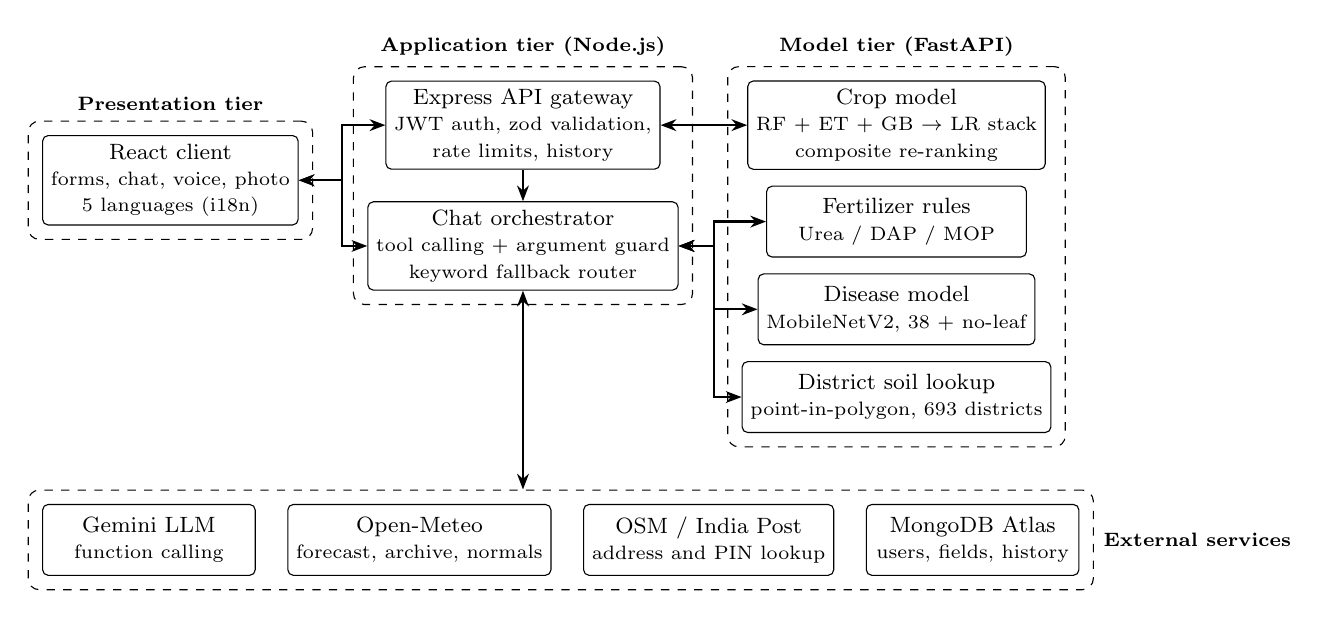
\begin{tikzpicture}[
  font=\footnotesize,
  box/.style={draw, rounded corners=2pt, align=center, minimum height=9mm, inner sep=3pt, fill=white},
  tier/.style={draw, dashed, rounded corners=4pt, inner sep=5pt},
  arr/.style={-{Stealth[length=2mm]}, thick},
  darr/.style={{Stealth[length=2mm]}-{Stealth[length=2mm]}, thick}
]
% client
\node[box, minimum width=3.0cm] (ui) {React client\\{\scriptsize forms, chat, voice, photo}\\{\scriptsize 5 languages (i18n)}};
% gateway
\node[box, right=1.1cm of ui, minimum width=3.2cm, yshift=7mm] (api) {Express API gateway\\{\scriptsize JWT auth, zod validation,}\\{\scriptsize rate limits, history}};
\node[box, below=4mm of api, minimum width=3.2cm] (orc) {Chat orchestrator\\{\scriptsize tool calling + argument guard}\\{\scriptsize keyword fallback router}};
% ml
\node[box, right=1.1cm of api, minimum width=3.3cm, yshift=0mm] (crop) {Crop model\\{\scriptsize RF + ET + GB $\rightarrow$ LR stack}\\{\scriptsize composite re-ranking}};
\node[box, below=2mm of crop, minimum width=3.3cm] (fert) {Fertilizer rules\\{\scriptsize Urea / DAP / MOP}};
\node[box, below=2mm of fert, minimum width=3.3cm] (dis) {Disease model\\{\scriptsize MobileNetV2, 38 + no-leaf}};
\node[box, below=2mm of dis, minimum width=3.3cm] (soil) {District soil lookup\\{\scriptsize point-in-polygon, 693 districts}};
% external services: one row below, reached only from the application tier
\node[box, minimum width=2.7cm, anchor=north west] (gem) at ($(ui.west |- soil.south)+(0,-0.9)$) {Gemini LLM\\{\scriptsize function calling}};
\node[box, right=4mm of gem, minimum width=2.7cm] (wx) {Open-Meteo\\{\scriptsize forecast, archive, normals}};
\node[box, right=4mm of wx, minimum width=2.7cm] (geo) {OSM / India Post\\{\scriptsize address and PIN lookup}};
\node[box, right=4mm of geo, minimum width=2.7cm] (db) {MongoDB Atlas\\{\scriptsize users, fields, history}};
% tiers
\begin{scope}[on background layer]
\node[tier, fit=(ui), label={[font=\scriptsize\bfseries]above:Presentation tier}] {};
\node[tier, fit=(api)(orc), label={[font=\scriptsize\bfseries]above:Application tier (Node.js)}] {};
\node[tier, fit=(crop)(soil), label={[font=\scriptsize\bfseries]above:Model tier (FastAPI)}] {};
\node[tier, fit=(gem)(db), label={[font=\scriptsize\bfseries]right:External services}] (ext) {};
\end{scope}
% arrows
\draw[darr] (ui.east) -- ++(0.55,0) |- (api.west);
\draw[darr] (ui.east) -- ++(0.55,0) |- (orc.west);
\draw[arr] (api.south) -- (orc.north);
\draw[darr] (api.east) -- (crop.west);
\draw[darr] (orc.east) -- ++(0.45,0) |- (dis.west);
\draw[darr] (orc.east) -- ++(0.45,0) |- (fert.west);
\draw[darr] (orc.east) -- ++(0.45,0) |- (soil.west);
\draw[darr] (orc.south) -- (orc.south |- ext.north);
\end{tikzpicture}
\caption{System architecture. The client talks only to the Express gateway. The gateway calls the model service with an internal key and is the only component that contacts Gemini, the weather and address services and the database.}
\label{fig:arch}
\end{figure*}

\subsection{Architecture of the System}
Fig.~\ref{fig:arch} shows the three tiers and the external services. The main software components are as follows.

\textit{1) React Client:} A single-page application built with React~18 and Vite. All interface text is stored in translation files with the same set of keys for every language, and the selected language is saved in the user profile. The chat screen supports browser speech input, photo upload and cards that display the structured result of each tool call next to the assistant's text.

\textit{2) Express API Gateway:} A Node.js server issues JSON Web Tokens, validates every request body with schema checks, applies per-user rate limits and saves predictions to MongoDB. It is the only component that holds secrets, and it adds an internal key header when it calls the model service, so the model service cannot be used directly from outside.

\textit{3) FastAPI Model Service:} A Python service loads all trained artifacts once at start-up. If one artifact is missing, only that feature is switched off and the health endpoint reports a degraded state; the other features keep working. Every response carries a \texttt{model\_version} field and confidence values.

\textit{4) Chat Orchestrator:} The orchestrator sends the farmer's message, a short history and five tool declarations (crop, location-based crop, fertilizer, disease and weather) to a Gemini model. The model name is read from configuration; the reported runs used \texttt{gemini-3.1-flash-lite} with minimal reasoning because it offered the most generous free quota. At most three tool rounds are allowed per message, after which the model must reply in text.

\textit{5) Data and External Services:} Weather forecasts, 30-day rainfall history and ten-year climate normals come from the Open-Meteo API \cite{openmeteo}. Address search and reverse geocoding use OpenStreetMap services, and PIN codes are resolved through the India Post directory. Users, fields, soil tests, crop history, chat sessions and predictions are stored in MongoDB.

\subsection{Data Collection and Model Training}

\textit{1) Crop Dataset:} We used the public Crop Recommendation dataset \cite{ingle2020}, which contains 2,200 records of 22 crops (100 per crop). Each record has seven features,
\begin{equation}
\mathbf{x} = [N,\; P,\; K,\; T,\; H,\; pH,\; R],
\label{eq:x}
\end{equation}
where $N$, $P$ and $K$ are the soil nutrient values, $T$ is temperature in $^{\circ}$C, $H$ is relative humidity in percent and $R$ is rainfall in millimetres. An initial audit found no missing values and no duplicate rows. Labels were integer-encoded, and features were standardised with a scaler fitted on the training part only. The data were divided by a stratified 80/20 split (seed 42) into 1,760 training and 440 test records. The test records were kept aside until the final evaluation.

\textit{2) Stacked Ensemble:} The ensemble uses three base learners: a Random Forest with 300 trees, an Extra Trees model with 300 trees and a stochastic Gradient Boosting model (150 stages, depth 3, learning rate 0.1, subsample 0.8). Let $\mathbf{p}_m(\mathbf{x}) \in [0,1]^{C}$ be the class-probability vector of base model $m$ for $C = 22$ crops. The meta-learner is a multinomial Logistic Regression applied to the concatenated vectors,
\begin{equation}
\hat{\mathbf{p}}(\mathbf{x}) = \operatorname{softmax}\!\big(W\,[\mathbf{p}_{\mathrm{RF}};\, \mathbf{p}_{\mathrm{ET}};\, \mathbf{p}_{\mathrm{GB}}] + \mathbf{b}\big).
\label{eq:stack}
\end{equation}
To prevent leakage, the meta-learner is fitted only on out-of-fold probabilities produced by a stratified five-fold split inside the training set. The base models are then refitted on the full training set. For comparison, four baselines were trained on identical splits: Decision Tree, Random Forest, Logistic Regression and an RBF-kernel SVM ($C = 10$).

\textit{3) Disease Images:} The disease module uses the colour PlantVillage images \cite{hughes2015} in the version without augmentation published on Mendeley Data \cite{pandian2019}: 54,305 leaf photographs in 38 classes covering 14 crops, plus 1,143 photographs that contain no leaf. The non-leaf photographs form a 39th class, so that a picture of soil, a hand or a wall is answered with a request for a new photograph instead of a diagnosis. The images are split 80/10/10 into training, validation and test sets, stratified by class, and resized to $224 \times 224$. Because the development machine has no GPU, training follows a two-step transfer-learning scheme. A MobileNetV2 backbone \cite{sandler2018} with ImageNet weights, frozen and preceded by a layer that rescales pixels to $[-1, 1]$, is run once over every image, and its 1,280-dimensional globally pooled features are cached. A head made of dropout (0.3) and a softmax layer is then trained on these features with Adam at a learning rate of $10^{-3}$, early stopping on validation accuracy and learning-rate reduction on plateau. Finally the head is attached to the backbone and exported as one model that accepts raw RGB images. A GPU notebook that also fine-tunes the top 30 backbone layers is included with the code, but it was not used for the results reported here. A curated knowledge file stores symptoms, organic and chemical treatments and prevention steps for all 38 classes.

\textit{4) District Soil Data:} For farmers without a soil report we compiled district statistics from the Government of India's Soil Health Card programme \cite{shc}, as published in a public GIS layer. The layer reports, for 779 districts and three recent years, the share of samples rated low, medium and high for $N$, $P$ and $K$, the share of acidic, neutral and alkaline samples, and the sample count. After removing districts with no data or fewer than ten samples, 693 districts remained. District boundaries were simplified to about 1~km so that a field location can be matched to its district by a point-in-polygon test.

\begin{figure}[t]
\centering
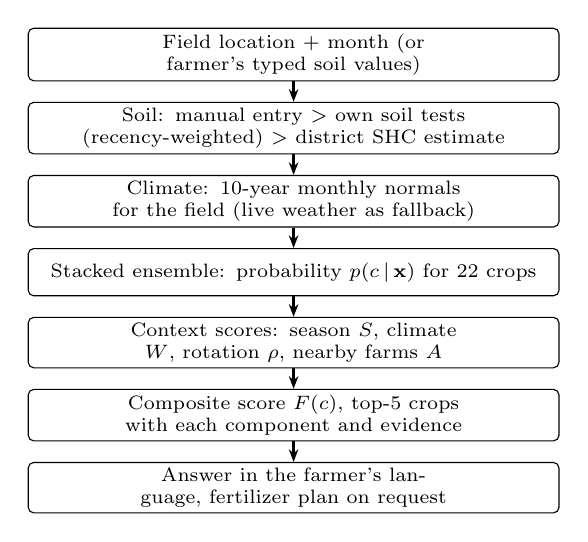
\begin{tikzpicture}[
  font=\scriptsize,
  st/.style={draw, rounded corners=2pt, align=center, text width=6.6cm, minimum height=6mm, inner sep=2pt},
  arr/.style={-{Stealth[length=1.6mm]}, thick},
  node distance=2.6mm
]
\node[st] (a) {Field location + month (or farmer's typed soil values)};
\node[st, below=of a] (b) {Soil: manual entry $>$ own soil tests (recency-weighted) $>$ district SHC estimate};
\node[st, below=of b] (c) {Climate: 10-year monthly normals for the field (live weather as fallback)};
\node[st, below=of c] (d) {Stacked ensemble: probability $p(c\,|\,\mathbf{x})$ for 22 crops};
\node[st, below=of d] (e) {Context scores: season $S$, climate $W$, rotation $\rho$, nearby farms $A$};
\node[st, below=of e] (f) {Composite score $F(c)$, top-5 crops with each component and evidence};
\node[st, below=of f] (g) {Answer in the farmer's language, fertilizer plan on request};
\draw[arr] (a) -- (b); \draw[arr] (b) -- (c); \draw[arr] (c) -- (d);
\draw[arr] (d) -- (e); \draw[arr] (e) -- (f); \draw[arr] (f) -- (g);
\end{tikzpicture}
\caption{Workflow of a location-based crop recommendation.}
\label{fig:flow}
\end{figure}

\subsection{Methodology}

Fig.~\ref{fig:flow} summarises how a recommendation is produced. The individual steps are described below.

\textit{1) Climate Fit:} For each crop $c$ and each climate variable $v \in \{T, H, R\}$, the mean $\mu_{c,v}$ and standard deviation $\sigma_{c,v}$ were computed from the training data. With $z = |v - \mu_{c,v}| / \sigma_{c,v}$, the fit of one variable is
\begin{equation}
f(z) = \min\!\Big(1,\; \max\!\Big(0,\; 1 - \frac{z - 1}{2}\Big)\Big),
\label{eq:fit}
\end{equation}
which equals one inside one standard deviation and falls linearly to zero at three. The climate score $W(c)$ is the mean of $f$ over the three variables. The dataset's rainfall column is on a monthly scale, so forecast rainfall is never used directly. Instead, the server supplies the observed rainfall of the last 30 days, or the long-term normal for the month when a field is selected.

\textit{2) Season Fit:} Each crop is tagged with the Indian seasons in which it is sown (Kharif, Rabi, Zaid). With three seasons every season borders the other two, so ``adjacent'' was defined as the \emph{upcoming} season:
\begin{equation}
S(c) = \begin{cases} 1.0 & \text{if $c$ is sown in the current season,}\\ 0.5 & \text{if $c$ is sown in the next season,}\\ 0 & \text{otherwise.}\end{cases}
\label{eq:season}
\end{equation}

\textit{3) Composite Score:} The base ranking combines the three signals with fixed weights,
\begin{equation}
F_0(c) = 0.6\,p(c\,|\,\mathbf{x}) + 0.2\,S(c) + 0.2\,W(c).
\label{eq:base}
\end{equation}
When the field has a crop history, a rotation score $\rho(c)$ is added. It is 0 for repeating last season's crop, 0.4 for a crop grown in the last three seasons, 1.0 for a legume after a non-legume, 0.8 for a different family, 0.5 for the same family and 0.5 for perennials. When at least five records from other farms within a set radius exist for the \emph{same season} in the last year, an area score $A(c) = n_c / \max_k n_k$ is also added, where $n_c$ is the number of records for crop $c$. Each active extra $j$ receives a weight $\omega_j = 0.1$, and the base weights are scaled down proportionally:
\begin{equation}
F(c) = \Big(1 - \sum_{j} \omega_j\Big) F_0(c) + \sum_{j} \omega_j\, X_j(c),
\label{eq:full}
\end{equation}
with $X_j \in \{\rho, A\}$. With both extras the weights become 0.48/0.16/0.16/0.10/0.10, and with no context (\ref{eq:full}) reduces exactly to (\ref{eq:base}). Each component is returned to the client and shown as a stacked bar, so the farmer and the LLM can see \emph{why} a crop ranks where it does.

\textit{4) Soil Estimation Hierarchy:} Values typed by the farmer always take priority. Otherwise, if the field has its own soil tests, each test $i$ taken $\Delta t_i$ days ago receives the weight $w_i = 2^{-\Delta t_i / 365}$, so a one-year-old test counts half as much as a new one, and
\begin{equation}
\hat{v} = \frac{\sum_i w_i\, v_i}{\sum_i w_i}.
\label{eq:recency}
\end{equation}
A least-squares slope over the test dates is also reported, so that a steady decline in, say, nitrogen is visible. If there are no tests, the district estimate is used. Since the Soil Health Card reports classes rather than values, the low, medium and high shares $(s_L, s_M, s_H)$ are mapped to the $1/6$, $1/2$ and $5/6$ quantiles of the training distribution,
\begin{equation}
\hat{v}_{\mathrm{dist}} = s_L\, q_{1/6} + s_M\, q_{1/2} + s_H\, q_{5/6},
\label{eq:district}
\end{equation}
and pH classes are mapped to 6.0, 7.0 and 8.0. For example, the quantiles for nitrogen are 14, 37 and 96. This yields a relative position on the model's own scale rather than a laboratory value, so the estimate's confidence is capped at 0.7 and decreases for small samples or mixed classes. The interface always labels such values as district estimates and advises a soil test.

\textit{5) Fertilizer Guidance:} The target for each nutrient is the mean value for the chosen crop in the training data. A value within $\pm 15\%$ of the target (and at least 5~kg/ha) is treated as adequate. Phosphorus is supplied first through DAP (18-46-0), whose nitrogen content is then credited, and urea and muriate of potash cover the rest:
\begin{equation}
\mathrm{DAP} = \frac{d_P}{0.46},\quad
\mathrm{Urea} = \frac{\max(0,\, d_N - 0.18\,\mathrm{DAP})}{0.46},\quad
\mathrm{MOP} = \frac{d_K}{0.60},
\label{eq:fert}
\end{equation}
where $d_X$ is the deficit of nutrient $X$ in kg/ha. Quantities are also shown per acre, together with organic alternatives, warnings for excess nutrients and a note to confirm with the local Krishi Vigyan Kendra. Because the rules are deterministic, the response carries no statistical confidence and is marked as rule-based.

\textit{6) Disease Screening:} Uploaded images are restricted to JPEG, PNG or WebP files of at most 5~MB, corrected for EXIF rotation and resized to $224 \times 224$. The service returns the top three classes. If the top probability is below 0.5, or if the no-leaf class wins, the result is marked as uncertain and the farmer is asked for a clearer photograph instead of being given a treatment. The no-leaf class is never shown as a diagnosis or among the top three. Every chemical recommendation includes a safety and label-dose disclaimer.

\textit{7) Guarded Tool Calling:} When Gemini requests a tool, the server does not run it immediately. Numeric soil and climate arguments are accepted only if the same number appears in the farmer's recent messages, after Indian-script digits are normalised to ASCII. Otherwise the tool returns a ``missing values'' result and the model has to ask the farmer. Leaf photographs are not sent to the LLM: the model receives only a short placeholder and calls the disease tool, which saves tokens and keeps images private. Each tool returns a compact summary for the model and a full result for the interface card.

\textit{8) Fallback Mode:} If the LLM times out (8~s per attempt, 15~s per message), returns a server error or reaches its quota, a keyword router takes over. It detects intent words, crop names in Latin and Indian scripts and $N$/$P$/$K$/pH values in all five languages, calls the same tools and fills language-specific templates. Tool results already obtained before the failure are reused, so no duplicate predictions are stored.

\textit{9) Weather Alerts:} Forecasts are converted to language-independent alert codes, including heavy rain ($\geq 64.5$~mm/day) and very heavy rain ($\geq 115.6$~mm/day) following IMD categories, heat ($\geq 40\,^{\circ}$C), frost ($\leq 4\,^{\circ}$C), strong wind, thunderstorms, a fungal-risk condition (humidity $\geq 85\%$ at 18--32~$^{\circ}$C) and dry spells. The client translates these codes, so alerts appear in the farmer's language without an extra LLM call.

\subsection{Challenges and Limitations}
Several limitations shape how the results should be read. The crop dataset is small, balanced and largely synthetic in character, so its near-perfect accuracy reflects clear class boundaries rather than proof of performance on real farms. It also omits several major Indian crops, such as wheat, sugarcane, mustard and soybean, which the fertilizer module therefore cannot serve. District soil estimates are coarse: a district can contain very different soils, and the class-to-quantile mapping preserves ordering but not true magnitudes. Climate inputs outside the training range, for example the near-zero rainfall of a southern Indian November, push the model towards drought-tolerant fruits; the season score reduces this effect but does not remove it. The disease network keeps its backbone frozen, so its accuracy is a few points below that of fully fine-tuned networks, and it was evaluated only on PlantVillage photographs of single leaves on plain backgrounds; field photographs with several leaves, shadows and soil are likely to score lower. Like any closed-set classifier, it can still give a confident label to an input unlike anything it was trained on, such as random noise. The no-leaf class catches ordinary non-leaf photographs, but not every unusual input. Finally, free-tier LLM quotas are small, which limits large-scale conversational testing.

% =============================================================================================
\section{Experimental Results}

The system was evaluated at five levels: the crop model alone, the leaf-disease model, the context-aware ranking on real locations, the multilingual conversational pipeline, and the software as a whole.

\subsection{Crop Model Comparison}
Table~\ref{tab:models} lists five-fold cross-validation accuracy on the training set and macro-averaged scores on the untouched test set. Fig.~\ref{fig:compare} plots the same numbers on a common axis.

\begin{table}[t]
\caption{Crop Recommendation Performance (Test $n = 440$)}
\label{tab:models}
\centering
\footnotesize
\setlength{\tabcolsep}{3.2pt}
\begin{tabular}{@{}lccccr@{}}
\toprule
\textbf{Model} & \textbf{CV Acc. (\%)} & \textbf{Acc.} & \textbf{Prec.} & \textbf{F1} & \textbf{Fit (s)}\\
\midrule
Decision Tree       & 98.52 $\pm$ 0.68 & 0.9795 & 0.9806 & 0.9794 & 0.03\\
Logistic Regression & 96.82 $\pm$ 0.66 & 0.9727 & 0.9740 & 0.9725 & 0.10\\
SVM (RBF)           & 98.24 $\pm$ 0.49 & 0.9886 & 0.9896 & 0.9887 & 0.07\\
Random Forest       & 99.32 $\pm$ 0.53 & 0.9955 & 0.9957 & 0.9955 & 1.23\\
\textbf{Stacked (ours)} & \textbf{99.43 $\pm$ 0.48} & \textbf{0.9955} & \textbf{0.9957} & \textbf{0.9955} & 231.99\\
\bottomrule
\multicolumn{6}{@{}p{0.95\columnwidth}@{}}{\scriptsize Prec., F1: macro averages over 22 classes; macro recall equals accuracy because the test set is balanced. Fit: training time on the full training set (CPU).}
\end{tabular}
\end{table}

\begin{figure}[t]
\centering
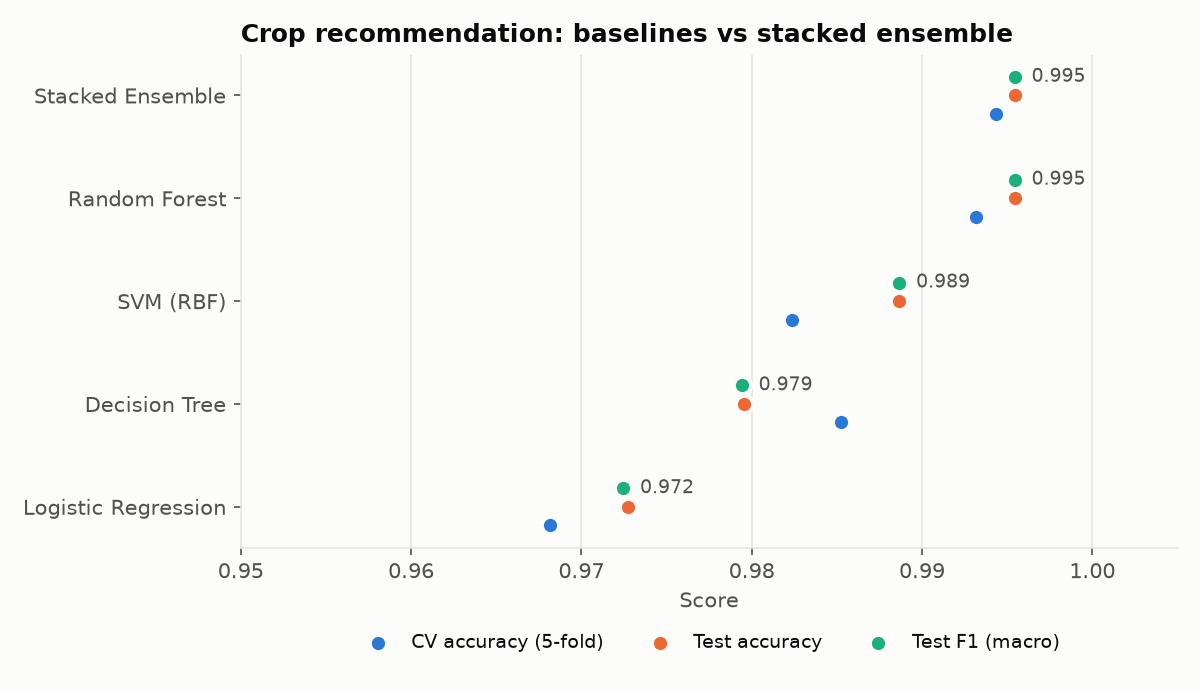
\includegraphics[width=\columnwidth]{model_comparison.png}
\caption{Cross-validation accuracy, test accuracy and test macro-F1 for each model. The axis starts at 0.95 to separate the closely spaced models.}
\label{fig:compare}
\end{figure}

The stacked ensemble and Random Forest tie on the test set, each misclassifying 2 of 440 samples. The ensemble, however, has the highest cross-validation mean and the lowest variance across folds (0.48 points), which suggests that it is the more stable choice when the training data change. Its cost is training time: about 232~s against 1.2~s for Random Forest, mainly because Gradient Boosting fits one tree per class at every stage. Training is done offline, and a single prediction takes a few milliseconds, so this cost does not affect users. Logistic Regression is the weakest model, which is expected because several crops are separated by non-linear boundaries in humidity and rainfall.

\subsection{Error Analysis and Feature Importance}
The two test errors of the ensemble were a blackgram sample labelled as maize and a lentil sample labelled as moth bean. Both pairs are rain-fed crops grown in similar nutrient and temperature ranges, so the confusion is agronomically plausible. Fig.~\ref{fig:importance} shows the permutation importance on the test set. Humidity (0.376) and rainfall (0.324) dominate, followed by $N$, $P$ and $K$ (0.13--0.18), while pH and temperature have almost no effect (below 0.01). This ranking has a practical consequence: the quality of the humidity and rainfall inputs matters far more than that of temperature. It is the reason the system uses observed rainfall and long-term normals instead of a single day's forecast.

\begin{figure}[t]
\centering
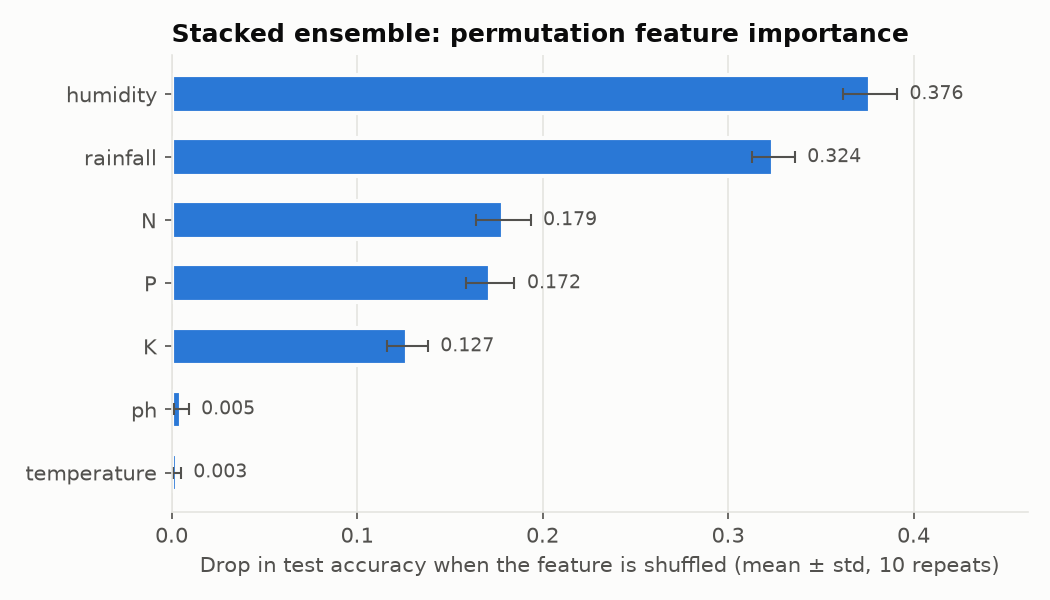
\includegraphics[width=\columnwidth]{feature_importance.png}
\caption{Permutation feature importance of the stacked ensemble (mean $\pm$ std over 10 repeats).}
\label{fig:importance}
\end{figure}

\subsection{Leaf Disease Model}
Table~\ref{tab:disease} reports the disease network on the held-out test set of 5,545 images. Feature extraction over all 55,448 images took about 30 minutes on a four-core laptop CPU (Intel Core i7-1165G7), and the head trained in about 35~s, stopping after 39 epochs (Fig.~\ref{fig:dcurves}). The correct class was among the top three predictions for 99.6\% of the test images, and only 1.2\% of them fell below the 0.5 confidence threshold at which the service withholds a treatment. Ten of the 39 classes were classified without error and 22 reached an F1 score of at least 0.98. The weakest classes were leaf-spot diseases with similar lesions, mostly on tomato: early blight (F1 0.80), target spot (0.87), maize grey leaf spot (0.87), tomato mosaic virus (0.88) and Septoria leaf spot (0.90). The no-leaf class rejected all 115 non-leaf test photographs (recall 1.00, precision 0.99). These scores are below the figures above 99\% reported for fully fine-tuned networks \cite{mohanty2016,too2019}, which is the expected cost of a frozen backbone trained without a GPU. Like those results, they were measured on laboratory-style photographs.

\begin{table}[t]
\caption{Leaf Disease Model (Test $n = 5{,}545$, 39 Classes)}
\label{tab:disease}
\centering
\footnotesize
\begin{tabular}{@{}lr@{}}
\toprule
\textbf{Metric} & \textbf{Value}\\
\midrule
Accuracy                         & 0.9688\\
Macro precision                  & 0.9639\\
Macro recall                     & 0.9609\\
Macro F1                         & 0.9622\\
Top-3 accuracy                   & 0.9960\\
Share below 0.5 confidence       & 1.21\%\\
No-leaf class precision / recall & 0.99 / 1.00\\
\bottomrule
\multicolumn{2}{@{}p{0.75\columnwidth}@{}}{\scriptsize Frozen ImageNet MobileNetV2 with a trained dropout and softmax head; stratified 80/10/10 split, seed 42.}
\end{tabular}
\end{table}

\begin{figure}[t]
\centering
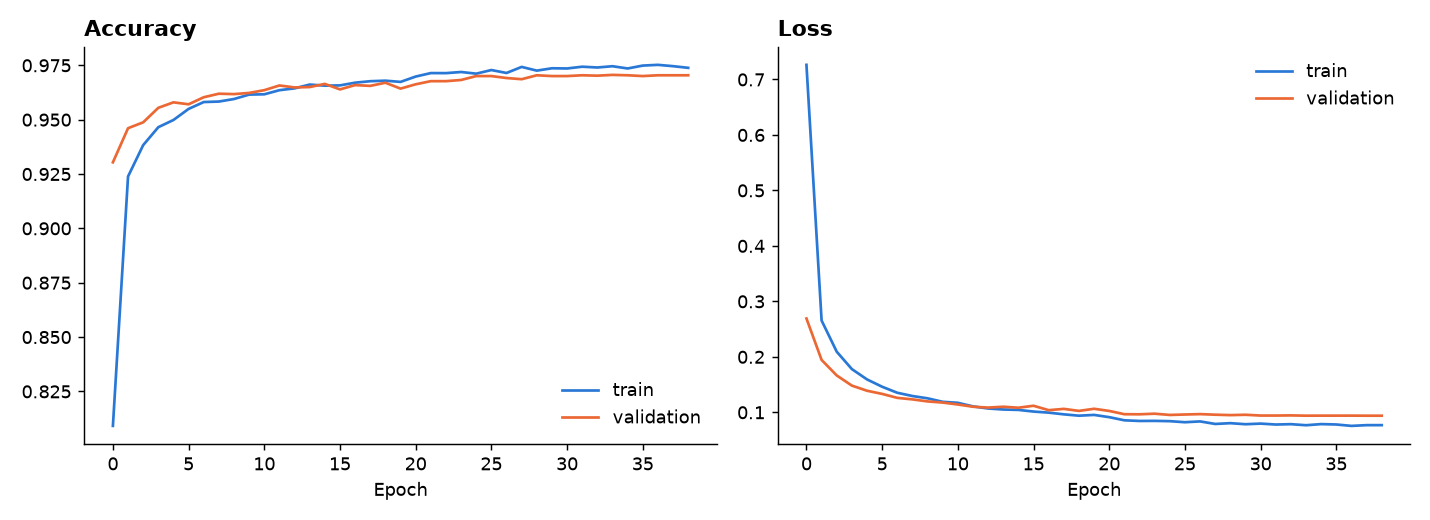
\includegraphics[width=\columnwidth]{disease_training_curves.png}
\caption{Training and validation accuracy and loss of the disease head.}
\label{fig:dcurves}
\end{figure}

\subsection{Context-Aware Ranking in Real Locations}
To check whether the composite score behaves sensibly, the full pipeline was run with real Open-Meteo climate data and the deployed model.
\begin{itemize}
\item \emph{Hyderabad, July (Kharif):} The ten-year July normals were 25.5~$^{\circ}$C, 79\% humidity and 231~mm of rainfall. Rice stayed at rank one with a model probability of 0.92, although the field's previous crop was also rice and the rotation score was therefore zero.
\item \emph{Nalgonda, November (Rabi), no soil test:} The district estimate gave $N = 14$, $P = 76$, $K = 32.6$ and pH 6.98, and lentil ranked first with a probability of 0.90.
\item \emph{Hyderabad, November, previous crop paddy:} Muskmelon ranked first on model probability (0.52) even though its climate fit was zero, and lentil followed with the full rotation score of 1.0 as a pulse after a cereal. With live November weather (30\% humidity, no rain), a rice-like soil scored a climate fit of only 0.14 for rice. This is the dry-season limitation discussed in Section~III-E.
\end{itemize}
On the soil side, 236 of the 676 districts with nitrogen data had at least 95\% of their samples rated low in nitrogen, consistent with the widespread nitrogen deficiency reported for Indian soils by the Soil Health Card programme \cite{shc}.

\subsection{Multilingual Conversational Evaluation}
Eight chat messages were sent through the complete stack (gateway API, orchestrator, Gemini, model service and MongoDB). Table~\ref{tab:chat} summarises the results. In one case the LLM was deliberately starved by setting its time budget to 1~ms, which forced the fallback path.

\begin{table}[t]
\caption{End-to-End Conversation Trial}
\label{tab:chat}
\centering
\footnotesize
\setlength{\tabcolsep}{2.6pt}
\begin{tabular}{@{}llllr@{}}
\toprule
\textbf{Lang.} & \textbf{Request} & \textbf{Tool called} & \textbf{Mode} & \textbf{Time (s)}\\
\midrule
Hindi    & Crop, soil values given      & recommendCrop       & AI    & 7.29\\
English  & Crop, pH missing             & recommendCrop$^{\ast}$ & AI & 2.50\\
English  & Follow-up with pH            & recommendCrop       & AI    & 5.19\\
Telugu   & Fertilizer for rice          & recommendFertilizer & AI    & 3.29\\
English  & Leaf photograph              & detectDisease$^{\dagger}$ & AI & 3.34\\
Tamil    & Weather and sowing           & getWeather          & AI    & 8.93\\
Kannada  & Crop (LLM forced to fail)    & recommendCrop       & Basic & 2.12\\
English  & Off-topic question           & none (declined)     & AI    & 1.90\\
\bottomrule
\multicolumn{5}{@{}p{0.95\columnwidth}@{}}{\scriptsize $^{\ast}$The LLM supplied pH = 7, which the farmer never typed; the guard rejected the call and the assistant asked for pH. $^{\dagger}$The disease model had not yet been trained when this trial was run; the service returned a clear ``unavailable'' message and the rest of the system continued to work.}
\end{tabular}
\end{table}

All eight messages reached the intended tool, or correctly reached no tool for the off-topic question. The median response time was 3.3~s (range 1.9--8.9~s). Most of this time is spent in the LLM: the crop model itself returns in milliseconds, and the slowest cases are those in which the model makes two calls, one to choose the tool and one to write the answer. The second message shows the value of the argument guard. The LLM silently filled in a neutral pH of 7, which would have produced a confident but unfounded recommendation. The guard detected that the value was absent from the conversation, and the assistant asked the farmer instead. In the forced-failure test the Kannada request, which carried the same soil values as the Hindi one, was answered in 2.1~s by the keyword router, which extracted the four numbers itself and called the same crop tool. The off-topic request was politely declined, as intended by the system prompt.

\subsection{Software Verification}
Correctness of the non-ML logic was checked with automated tests. The model service has 53 passing tests and one skipped test, covering scoring formulas, fertilizer arithmetic, image validation, the district lookup and degraded start-up. The gateway has 93 passing tests that run against an in-memory database and scripted fakes of the model service, the weather APIs, the geocoders and Gemini. These tests cover authentication, validation, the argument guard, time-outs, retries, fallback routing in all five languages and the location-based pipeline. In total, 146 tests passed and none failed.

\subsection{Comparison with Typical Approaches}
Table~\ref{tab:compare} contrasts the proposed system with the kinds of systems reviewed in Section~II. The accuracy of the crop model is similar to that of other ensemble recommenders on the same benchmark; the gains of this work are in coverage, grounding and robustness rather than in raw accuracy.

\begin{table}[t]
\caption{Capability Comparison}
\label{tab:compare}
\centering
\footnotesize
\setlength{\tabcolsep}{3pt}
\begin{tabular}{@{}lccc@{}}
\toprule
\textbf{Capability} & \textbf{Crop ML \cite{pudumalar2017}} & \textbf{Disease CNN \cite{mohanty2016}} & \textbf{This work}\\
\midrule
Crop recommendation         & \checkmark & --         & \checkmark\\
Season / rotation awareness & --         & --         & \checkmark\\
Works without soil report   & --         & --         & \checkmark\\
Fertilizer quantities       & --         & --         & \checkmark\\
Leaf disease screening      & --         & \checkmark & \checkmark\\
Indian-language chat        & --         & --         & \checkmark\\
LLM argument validation     & --         & --         & \checkmark\\
Works when LLM fails        & n/a        & n/a        & \checkmark\\
\bottomrule
\end{tabular}
\end{table}

% =============================================================================================
\section{Conclusion}

This paper presented a multilingual agriculture decision support system that brings crop recommendation, fertilizer planning, leaf-disease screening and weather alerts into one interface for Indian farmers. A stacked ensemble of tree models reached 99.55\% test accuracy and the most stable cross-validation score of the five models compared. The MobileNetV2 disease network, trained on a laptop CPU with a frozen backbone, classified 96.88\% of held-out PlantVillage images correctly and declined to diagnose photographs that contained no leaf. More importantly for practical use, its predictions are re-ranked by an explainable score that respects the sowing season, the local climate, the field's crop history and the crops grown nearby. A soil-estimation hierarchy based on personal tests and Soil Health Card statistics for 693 districts lets farmers without a laboratory report obtain a recommendation, with the uncertainty stated openly.

The conversational layer shows that a lightweight LLM can serve as a multilingual front end without being trusted with numbers. Restricting it to tool selection and wording, checking every argument against the farmer's own words, and keeping a rule-based fallback produced correct routing for all test messages in five languages, a median response time of 3.3~s, and the interception of a hallucinated soil value that would otherwise have reached the model.

Future work will proceed in four directions. First, the MobileNetV2 disease network will be fine-tuned on GPU hardware and evaluated on field photographs from local farms. Second, the crop dataset will be extended with region-specific records for wheat, sugarcane, mustard and soybean so that the fertilizer module covers more crops. Third, a field study with farmers and Krishi Vigyan Kendra staff will measure usability, comprehension of confidence values and agreement with expert advice. Finally, offline operation and SMS or voice-call access will be explored for areas with weak connectivity.

\section*{Acknowledgment}
The authors thank the Department of Computer Science and Engineering, Ajay Kumar Garg Engineering College, Ghaziabad, for providing the facilities and guidance for this work. We also acknowledge the open data made available by the Soil Health Card programme, Open-Meteo and the OpenStreetMap community.

% =============================================================================================
\begin{thebibliography}{00}

\bibitem{fabregas2019} R. Fabregas, M. Kremer, and F. Schilbach, ``Realizing the potential of digital development: The case of agricultural advice,'' \emph{Science}, vol. 366, no. 6471, Art. no. eaay3038, 2019, doi: 10.1126/science.aay3038.

\bibitem{pudumalar2017} S. Pudumalar, E. Ramanujam, R. H. Rajashree, C. Kavya, T. Kiruthika, and J. Nisha, ``Crop recommendation system for precision agriculture,'' in \emph{Proc. 8th Int. Conf. Advanced Computing (ICoAC)}, Chennai, India, 2017, pp. 32--36, doi: 10.1109/ICoAC.2017.7951740.

\bibitem{liakos2018} K. G. Liakos, P. Busato, D. Moshou, S. Pearson, and D. Bochtis, ``Machine learning in agriculture: A review,'' \emph{Sensors}, vol. 18, no. 8, Art. no. 2674, 2018, doi: 10.3390/s18082674.

\bibitem{mohanty2016} S. P. Mohanty, D. P. Hughes, and M. Salath\'e, ``Using deep learning for image-based plant disease detection,'' \emph{Frontiers in Plant Science}, vol. 7, Art. no. 1419, 2016, doi: 10.3389/fpls.2016.01419.

\bibitem{ferentinos2018} K. P. Ferentinos, ``Deep learning models for plant disease detection and diagnosis,'' \emph{Computers and Electronics in Agriculture}, vol. 145, pp. 311--318, 2018, doi: 10.1016/j.compag.2018.01.009.

\bibitem{ji2023} Z. Ji \emph{et al.}, ``Survey of hallucination in natural language generation,'' \emph{ACM Computing Surveys}, vol. 55, no. 12, pp. 1--38, 2023, doi: 10.1145/3571730.

\bibitem{tzachor2023} A. Tzachor \emph{et al.}, ``Large language models and agricultural extension services,'' \emph{Nature Food}, vol. 4, pp. 941--948, 2023, doi: 10.1038/s43016-023-00867-x.

\bibitem{breiman2001} L. Breiman, ``Random forests,'' \emph{Machine Learning}, vol. 45, no. 1, pp. 5--32, 2001, doi: 10.1023/A:1010933404324.

\bibitem{geurts2006} P. Geurts, D. Ernst, and L. Wehenkel, ``Extremely randomized trees,'' \emph{Machine Learning}, vol. 63, no. 1, pp. 3--42, 2006, doi: 10.1007/s10994-006-6226-1.

\bibitem{friedman2001} J. H. Friedman, ``Greedy function approximation: A gradient boosting machine,'' \emph{Annals of Statistics}, vol. 29, no. 5, pp. 1189--1232, 2001, doi: 10.1214/aos/1013203451.

\bibitem{wolpert1992} D. H. Wolpert, ``Stacked generalization,'' \emph{Neural Networks}, vol. 5, no. 2, pp. 241--259, 1992, doi: 10.1016/S0893-6080(05)80023-1.

\bibitem{hughes2015} D. P. Hughes and M. Salath\'e, ``An open access repository of images on plant health to enable the development of mobile disease diagnostics,'' \emph{arXiv preprint} arXiv:1511.08060, 2015.

\bibitem{too2019} E. C. Too, L. Yujian, S. Njuki, and L. Yingchun, ``A comparative study of fine-tuning deep learning models for plant disease identification,'' \emph{Computers and Electronics in Agriculture}, vol. 161, pp. 272--279, 2019, doi: 10.1016/j.compag.2018.03.032.

\bibitem{sandler2018} M. Sandler, A. Howard, M. Zhu, A. Zhmoginov, and L.-C. Chen, ``MobileNetV2: Inverted residuals and linear bottlenecks,'' in \emph{Proc. IEEE/CVF Conf. Computer Vision and Pattern Recognition (CVPR)}, 2018, pp. 4510--4520, doi: 10.1109/CVPR.2018.00474.

\bibitem{kamilaris2018} A. Kamilaris and F. X. Prenafeta-Bold\'u, ``Deep learning in agriculture: A survey,'' \emph{Computers and Electronics in Agriculture}, vol. 147, pp. 70--90, 2018, doi: 10.1016/j.compag.2018.02.016.

\bibitem{wolfert2017} S. Wolfert, L. Ge, C. Verdouw, and M.-J. Bogaardt, ``Big data in smart farming -- A review,'' \emph{Agricultural Systems}, vol. 153, pp. 69--80, 2017, doi: 10.1016/j.agsy.2017.01.023.

\bibitem{zhai2020} Z. Zhai, J. F. Mart\'{\i}nez, V. Beltran, and N. L. Mart\'{\i}nez, ``Decision support systems for agriculture 4.0: Survey and challenges,'' \emph{Computers and Electronics in Agriculture}, vol. 170, Art. no. 105256, 2020, doi: 10.1016/j.compag.2020.105256.

\bibitem{silva2023} B. Silva \emph{et al.}, ``GPT-4 as an agronomist assistant? Answering agriculture exams using large language models,'' \emph{arXiv preprint} arXiv:2310.06225, 2023.

\bibitem{lewis2020} P. Lewis \emph{et al.}, ``Retrieval-augmented generation for knowledge-intensive NLP tasks,'' in \emph{Advances in Neural Information Processing Systems (NeurIPS)}, vol. 33, 2020, pp. 9459--9474.

\bibitem{schick2023} T. Schick \emph{et al.}, ``Toolformer: Language models can teach themselves to use tools,'' in \emph{Advances in Neural Information Processing Systems (NeurIPS)}, vol. 36, 2023.

\bibitem{yao2023} S. Yao \emph{et al.}, ``ReAct: Synergizing reasoning and acting in language models,'' in \emph{Proc. Int. Conf. Learning Representations (ICLR)}, 2023.

\bibitem{gemini_fc} Google, ``Function calling with the Gemini API,'' Google AI for Developers. [Online]. Available: \url{https://ai.google.dev/gemini-api/docs/function-calling}

\bibitem{pedregosa2011} F. Pedregosa \emph{et al.}, ``Scikit-learn: Machine learning in Python,'' \emph{Journal of Machine Learning Research}, vol. 12, pp. 2825--2830, 2011.

\bibitem{openmeteo} P. Zippenfenig, ``Open-Meteo.com Weather API,'' Zenodo, 2023, doi: 10.5281/zenodo.7970649.

\bibitem{ingle2020} A. Ingle, ``Crop recommendation dataset,'' Kaggle, 2020. [Online]. Available: \url{https://www.kaggle.com/datasets/atharvaingle/crop-recommendation-dataset}

\bibitem{pandian2019} J. Arun Pandian and G. Geetharamani, ``Data for: Identification of plant leaf diseases using a 9-layer deep convolutional neural network,'' Mendeley Data, v1, 2019, doi: 10.17632/tywbtsjrjv.1.

\bibitem{shc} Department of Agriculture and Farmers Welfare, Government of India, ``Soil Health Card scheme portal.'' [Online]. Available: \url{https://soilhealth.dac.gov.in}

\end{thebibliography}

\end{document}
